\documentclass[10pt,a4paper]{article}
\usepackage[a4paper,margin=1.8cm]{geometry}
\usepackage[T1]{fontenc}
\usepackage{lmodern}
\usepackage{microtype}
\usepackage{booktabs}
\usepackage{tabularx}
\usepackage{array}
\usepackage[table]{xcolor}
\usepackage{enumitem}
\usepackage{titlesec}
\usepackage{url}
\usepackage[colorlinks=true,linkcolor=blue!50!black,urlcolor=blue!50!black]{hyperref}
\usepackage{graphicx}
\graphicspath{{issue-54-figs/}}
\setlength{\textfloatsep}{1.6ex plus 0.6ex}
\setlength{\floatsep}{1.4ex plus 0.6ex}
\renewcommand{\topfraction}{0.9}
\renewcommand{\textfraction}{0.08}
\renewcommand{\floatpagefraction}{0.85}
\newcommand{\figcap}[1]{\caption{\footnotesize #1}}

\setlist{nosep,leftmargin=1.3em}
\titlespacing*{\section}{0pt}{1.1ex}{0.6ex}
\titlespacing*{\subsection}{0pt}{0.9ex}{0.4ex}
\setlength{\parindent}{0pt}
\setlength{\parskip}{0.45ex}
\renewcommand{\arraystretch}{1.08}
\newcommand{\iss}[1]{\href{https://github.com/JieGH/RVV_code_gen_via_MLIR_xDSL/issues/#1}{\##1}}
\newcommand{\up}[1]{\textcolor{red!70!black}{#1}}
\newcommand{\down}[1]{\textcolor{blue!60!black}{#1}}
\newcommand{\good}[1]{\textcolor{green!45!black}{\textbf{#1}}}
\newcommand{\bad}[1]{\textcolor{red!70!black}{\textbf{#1}}}
\newcommand{\key}[1]{\textbf{\textcolor{blue!55!black}{#1}}}  % a key point

\title{\vspace{-1.2cm}\textbf{What in the B packer's reads sets off B3's slow state,\\ and a packer that keeps B3 steady}\\[2pt]
\large Brief of issue \iss{54} (spec \iss{55}), a follow-up of \iss{44}, \iss{48}, \iss{49}, \iss{50} and \iss{53}}
\author{RVV\_code\_gen\_via\_MLIR\_xDSL, \texttt{pure-xdsl}; branch \texttt{issue55-pack-b-variants}\\
SpacemiT X60 (RVV 1.0, VLEN 256), \texttt{jbpi2}; series 1 on 2026-10-22, series 2 on 2026-10-23}
\date{23 October 2026; figures added 29 October 2026}

\begin{document}
\maketitle
\vspace{-0.8cm}

\begin{center}
\fcolorbox{blue!50!black}{blue!4}{\parbox{0.96\textwidth}{\small
\textbf{Summary.} B3 (64$\times$384$\times$384) on the default 16$\times$15 tile runs at about 4.5 GOPs, because most reps
fall into a ``slow state'' in which pack and compute are both slower (\iss{48}, \iss{50}). We changed only the B packer,
behind a switch. Bc's layout, the microkernel, the blocking and the cache model stay fixed. There are eight read orders (the current one and seven
variants), and each writes a byte-identical Bc.

\textbf{Finding 1.} \key{The trigger is reading 4 bytes from each column of B per touch.} All three packers that do this (scalar loads
included) become slow on most 16$\times$8 and 16$\times$15 cells, and it happens even with no compute between packs. None of them
becomes slow on 16$\times$6 B3.

\textbf{Finding 2.} Reading one column at a time (\texttt{col-g1}, \texttt{col-g1-m4}) \key{gives no slow rep in any GEMM cell, on any
tile, K, board or night.} On the default tile, \key{B3 goes from 4.53--4.63 to 7.01--7.05 GOPs by mean time} (from 4.28 to
7.00--7.05 by median rep). B2 stays within 0.09 GOPs for \texttt{col-g1-m4} (0.21 for \texttt{col-g1}),
and Reuse24 no longer has slow reps.

\textbf{Finding 3.} Reading 2, 4 or all columns side by side removes the 4-byte trigger, but it brings back bad cells that depend
on tile and K, not on group size. It also brings a new state, ``steadily slow'' (\texttt{col-g2} at K=256).}}
\end{center}

\noindent\textit{Key points are in} \key{dark blue bold}\textit{.}

\paragraph{How the numbers were taken.} Every speed number is from the uninstrumented build (\texttt{INSTRUMENTED=0}), reference
protocol, \texttt{-{}-tmin 10}, core 4, \texttt{-{}-no-nc-overrides}, 3 launches per case, left rotation, on the board
\texttt{jbpi2}. A rep is one repetition of the timed call. Speed is in GOPs, by mean time (the reference's formula) and by median rep; ``slow \%'' is the share of reps in the slow state.
The secondary board \texttt{jbpi} was run in series 1 as a cross-check only. No board counters were read.

\section{Background}
B is column-major. Bc holds NR-wide panels, row-major inside a panel: element $(k,j)$ of panel $p$ sits at
\texttt{Bc[p*NR*kc + k*NR + j]}. The current xDSL packer does, for each k, one strided \texttt{vlse32} that gathers 8 columns.
At K=384 the stride is $\texttt{ldb}\cdot 4 = 1536$ B (\texttt{ldb} = 384 numbers between the starts of two columns, times 4 bytes per
fp32 number), so \key{each instruction touches 8 cache lines and takes 4 B from each.}

What the earlier issues found: the slow state follows NR (\iss{48}); the scalar packer is steadier but not cheaper (\iss{53});
padding \texttt{ldb} changes the state, but not in a simple pattern (\iss{49}); and slow reps halve the L1D prefetch hits (\iss{50}).
The X60 has no Zicbop and its prefetcher is undocumented. So this work changes the read pattern that the prefetcher sees, and
observes the result.

\paragraph{The sizes that matter (Figure~\ref{fig:units}).} A vector register is VLEN\,=\,256 bit, so it holds 8 fp32 lanes; RVV has
32 of them, and LMUL\,=\,4 joins four into one 128 B group of 32 lanes. The cache model's \texttt{jbpi2} config gives a 32 KB L1D
(128 sets $\times$ 4 ways $\times$ 64 B lines) and a 512 KB L2 (1024 sets $\times$ 8 ways $\times$ 64 B). B3's B is 384$\times$384 fp32
= 576 KB; one column is 1536 B = 24 lines, and one line holds 16 consecutive k of one column. The blocking in these runs is
mc\,=\,64, nc\,=\,384, and kc\,=\,256 at 16$\times$6 and 16$\times$8, 128 at 16$\times$15 (from the per-rep files). So one Bc block is
384 KB at 16$\times$6 and 16$\times$8 (64 or 48 panels), and 195 KB at 16$\times$15 (26 panels of 15$\times$128 floats = 7.5 KB each):
always larger than L1D and within L2.

\paragraph{Reading the numbers 4 and 8.} One load of the current packer fills one vector register with 8 numbers; each
number is one fp32 value of 4 bytes, and each comes from a different column of B. So one load takes 4 B from each of 8 columns,
32 B in total, from 8 different cache lines. In the figures, ``8'' always counts numbers, columns or cache lines, never bytes.

\paragraph{The different 4s in the code.} The number 4 appears in the code with two different meanings, which are easy to confuse:
\begin{center}\footnotesize\setlength{\tabcolsep}{5pt}
\begin{tabular}{@{}lp{11.2cm}@{}}
\toprule
where & what the 4 means \\
\midrule
\texttt{ldb * 4} (load of the current packer) & 4 \textbf{bytes} per fp32 number. \texttt{ldb} counts numbers (384 for B3), and the
instruction wants its stride in bytes: $384 \times 4 = 1536$ B between two numbers of one load. It does not mean ``4 elements'': the
load still reads 8 numbers. \\
\texttt{RR * 4} (store of the fix) & also 4 bytes per number: one row of the Bc panel is NR numbers, so the next row starts
$\mathrm{NR} \times 4$ bytes later (60 B at NR\,=\,15). \\
\texttt{m4}, LMUL\,=\,4 (load of the fix) & 4 \textbf{vector registers} joined into one long register. One register holds 8 numbers,
so four hold 32: one load reads 32 numbers. \\
``4 B from each column'' (in the text) & one fp32 number is 4 bytes. \\
\bottomrule
\end{tabular}
\end{center}

\begin{figure}[!htb]
\centering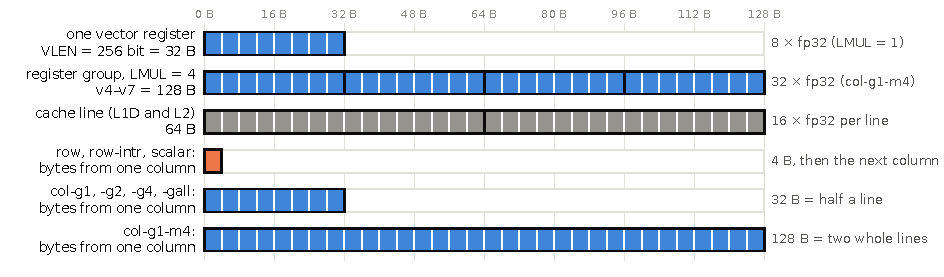
\includegraphics[width=\textwidth]{fig_units.pdf}
\figcap{Register, cache line and touch sizes, drawn to one byte scale. One cell is one fp32 (4 B). The bottom three rows are what one
touch of one column of B takes under each read order (property C).}
\label{fig:units}
\end{figure}

\section{The three properties and the variants}
A read order has three properties: (A) how a read is issued (strided vector, scalar, or unit-stride vector); (B) how many columns are
read side by side; (C) how many bytes are taken from one column per touch. Each variant changes these, and only these.
All variants write the same Bc: a host test compares them byte for byte, and the board test (5400 cases) has bad\,=\,0.
\texttt{col-gall} reads up to 24 columns at once; NR is at most 24 here, so it means NR.

\begin{center}\footnotesize\setlength{\tabcolsep}{4pt}
\begin{tabular}{@{}lp{5.6cm}lcc@{}}
\toprule
variant & how B is read & A: issue & B: columns at once & C: bytes per column \\
\midrule
\texttt{row} (current, xDSL) & \texttt{vlse32} across 8 columns per k & strided vector & NR & 4 \\
\texttt{row-intr} & the same, written as C intrinsics & strided vector & NR & 4 \\
\texttt{scalar} & one element at a time & scalar & NR & 4 \\
\texttt{col-gall} & \texttt{vle32} of 8 floats down each column, all NR columns side by side, then strided stores into Bc & unit-stride vector & NR & 32 \\
\texttt{col-g4} & the same, 4 columns at a time & unit-stride vector & 4 & 32 \\
\texttt{col-g2} & the same, 2 columns at a time & unit-stride vector & 2 & 32 \\
\texttt{col-g1} & one column at a time (the order \iss{44} asked for) & unit-stride vector & 1 & 32 \\
\texttt{col-g1-m4} & one column at a time, LMUL\,=\,4: 32 floats per load & unit-stride vector & 1 & 128 (two whole lines) \\
\bottomrule
\end{tabular}
\end{center}
\texttt{row-intr} is a control: it should behave like \texttt{row}. If it does not, the C path itself changes something (see Caveats).

\paragraph{The fix, and why it cannot change the result (Figure~\ref{fig:fixflow}).} A packer only copies numbers; it does no
arithmetic. Every read order puts each number of B at the same place in Bc, \texttt{Bc[k*NR + j] = B(k, j)}; only the order of the
copies differs. The current packer loads one row of B (8 numbers, one per column) into one register and stores it as one row of Bc.
The fix loads 32 numbers of one column into four joined registers (LMUL\,=\,4) and stores them down one column of Bc. When the panel is
done, \key{both Bc are the same byte for byte}, so the microkernel gets the same input, does the same arithmetic in the same order, and
gives the same C, bit for bit. This was checked, not only argued:
\begin{itemize}
  \item \textbf{Layout, host:} \texttt{test\_pack\_b\_variants.py} compares every variant with the scalar packer byte for byte (NR 1 to 31,
  partial panels, kc tails, \texttt{ldb} > kc, pad slots left as they were). A planted bug (the 32-number strip not cut at the end of a
  column) made it fail.
  \item \textbf{Layout, board} (\texttt{jbpi2}, GCC 13.2, \texttt{-O2} and \texttt{-O3}): the same harness on the real RVV code,
  5400 cases (6 variants $\times$ 10 NR $\times$ 5 kc $\times$ 6 nc $\times$ 3 \texttt{ldb}), 0 bad.
  \item \textbf{Full GEMM, board:} each of the 6 variants on 16$\times$15, on B3 and B3\_K256, with the result checked against the
  reference: 12 of 12 PASS.
  \item \textbf{Every pack-only run of both series} replays the packing with the scalar packer and compares the whole Bc: 108 of 108
  runs \texttt{ok}.
\end{itemize}
One limit: the timed GEMM runs of Tables 1--4 skip the result check (it would slow the timing loop); their correctness rests on the
checks above.

\paragraph{Why the fix does not slow anything else down.} Changing the read order could in principle cost speed in three places. \key{None
of them shows a loss.}
\begin{itemize}
  \item \textbf{The microkernel.} It reads Bc, not B, and Bc is the same byte for byte, in the same place. So the microkernel does the
  same loads and the same arithmetic as before. The fix changes only the packing step, and through it whether the run falls into the
  slow state (which slows both pack and compute, \iss{50}).
  \item \textbf{The scattered stores into Bc.} The fix exchanges scattered reads of B for scattered writes into Bc (one number every 60 B
  at 16$\times$15). This is the cheaper side: the writes all land inside the panel being filled, 7.5 KB at 16$\times$15 (120 lines),
  which fits easily in the 32 KB L1D, so the 15 column passes come back to lines that are most likely still in L1. The reads of B, by
  contrast, come from a 576 KB matrix that is not in L1. Measured cost: a fast pack takes 0.8218 ms against 0.6443 ms for
  \texttt{row-intr} (16$\times$15, B3, Table 3). But the fix never becomes slow, so its average pack is cheaper: 0.822 ms against
  1.155 ms (Figure~\ref{fig:packcost}).
  \item \textbf{Shapes that were never slow.} B2 and Reuse24 have no slow state to remove, so they show only the cost side. B2 stays
  within 0.09 GOPs of \texttt{row} with \texttt{col-g1-m4} (Table 4), inside the run-to-run spread. Reuse24 is the same or slightly
  better at 16$\times$6 and 16$\times$8 (9.29 against 9.21, 9.15 against 8.95), and better at 16$\times$15 (8.87 against 8.48), where
  \texttt{row} has 14--17\% slow reps. On B3 at 16$\times$6, where \texttt{row} is also
  never slow, the fix is slightly faster (6.89 against 6.72 GOPs).
\end{itemize}
The reason ``L1 hits on the stores'' is the likely one, not a measured one: these runs read no counters.

\begin{figure}[!htb]
\centering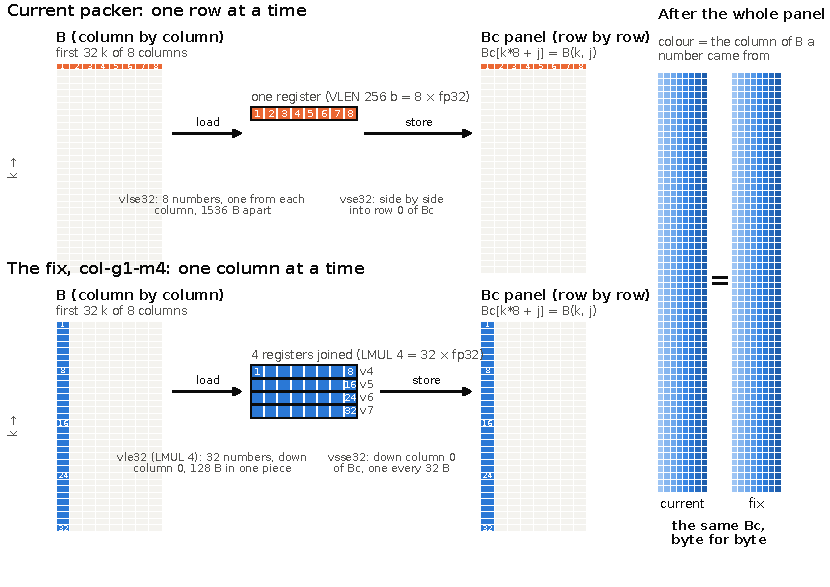
\includegraphics[width=\textwidth]{fig_fix_dataflow.pdf}
\figcap{One load and one store of the current packer (top) and of the fix (bottom), from B through the vector register(s) into Bc;
drawn for NR\,=\,8 and the first 32 k of a panel. The numbers show which register lane each value passes through. Right: the finished
panel, each number coloured by the column of B it came from: the same for both.}
\label{fig:fixflow}
\end{figure}

\paragraph{The fix at the C code level (Figure~\ref{fig:codediff}).} The fix changes three places of the packer and nothing else:
\textbf{(1)} the loop order, from ``k outside, columns inside'' to ``column outside, k inside''; \textbf{(2)} the load, from a strided
\texttt{vlse32} of 8 numbers (stride \texttt{ldb*4} = 1536 B) to a unit-stride \texttt{vle32} of 32 numbers (LMUL\,=\,4); \textbf{(3)} the
store, from a unit-stride \texttt{vse32} into a row of Bc to a strided \texttt{vsse32} down a column of Bc (stride \texttt{RR*4}). The
destination of every number, \texttt{Bp + i*RR + c} against \texttt{Bp + i*RR + jj}, is the same element of Bc.
Note on the 4s: in \texttt{ldb*4} and \texttt{RR*4} the 4 is the size of one fp32 number in bytes (the intrinsics take strides in
bytes), so \texttt{ldb*4} = 384 numbers $\times$ 4 B = 1536 B; it is not a count of elements. In \texttt{m4} (LMUL\,=\,4) the 4 is the
number of vector registers joined together: 4 registers of 8 numbers = 32 numbers per load.

\begin{figure}[!htb]
\centering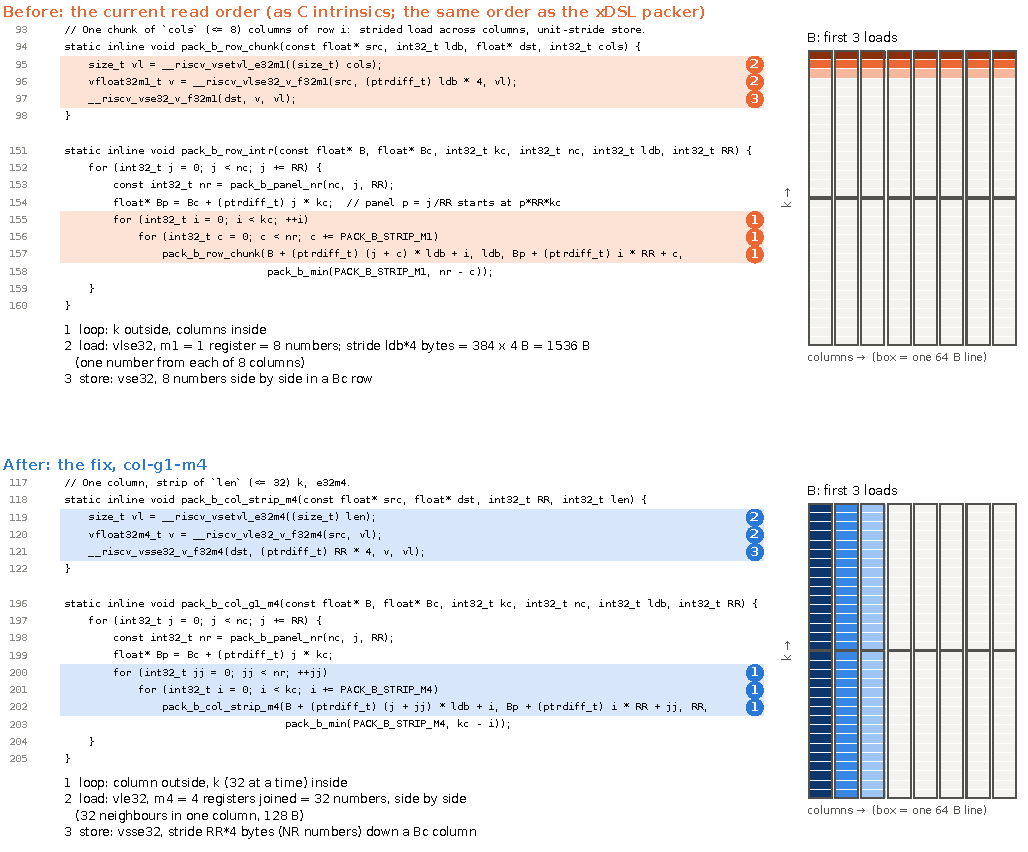
\includegraphics[width=\textwidth]{fig_code_diff.pdf}
\figcap{Before and after, as C intrinsics, verbatim from \texttt{tests/pure\_xdsl\_blis\_rvv/templates/pack\_b\_variants.h} (line numbers
on the left). ``Before'' is the current read order written as C (\texttt{row-intr}, the same loop as the xDSL packer of Appendix~C.2--C.3);
``after'' is the fix. The marked lines are the three changes: 1 the loop order, 2 the load, 3 the store. In \texttt{ldb * 4} and
\texttt{RR * 4} the 4 is bytes per fp32 number (a stride in bytes); in \texttt{m4} it is 4 registers joined (32 numbers). Right: the first three loads
each version issues on B (dark, mid, light), drawn for 8 columns and 32 k; one box is one 64 B cache line.}
\label{fig:codediff}
\end{figure}

\paragraph{What each order asks of memory (Figures~\ref{fig:order} and~\ref{fig:counts}).} Counted from the loop nests, for one full
panel of B3 on the default tile (NR\,=\,15, kc\,=\,128: 1920 floats, 7.5 KB, 120 lines of B). The current order issues 256 strided
loads (8\,+\,7 lanes per k); each touches 7 or 8 lines of B and takes 4 B from each, so all 15 columns are open at once and every B
line is visited 16 times, once per k. \texttt{col-g1-m4} issues 60 loads; each takes two whole lines from one column, so one column is
open at a time and every B line is visited once. The cost moves to the store side: a strided store of \texttt{col-g1-m4} spreads its
32 floats over 30 lines of Bc (stride 60 B), against 1--2 lines for the unit-stride store of \texttt{row}. The runs in
\S\ref{sec:packonly} show that this exchange is worth it.

\begin{figure}[!htb]
\centering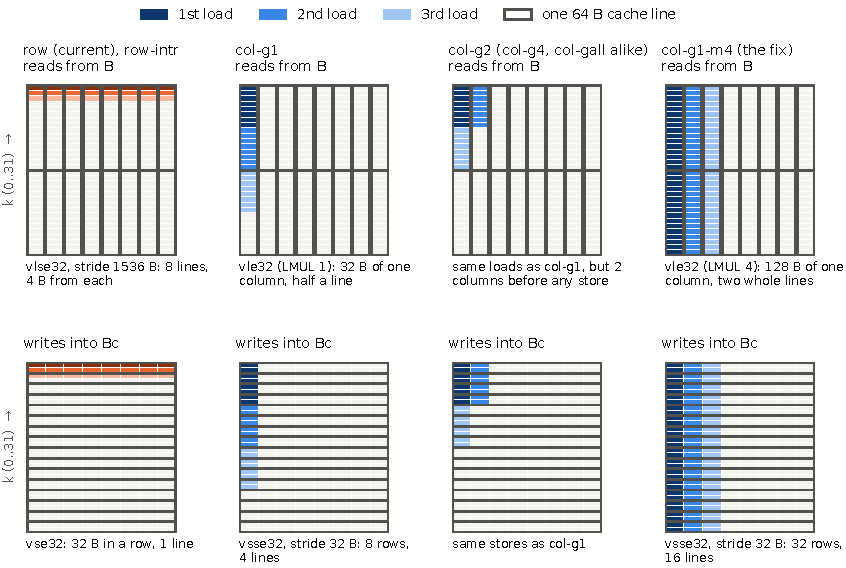
\includegraphics[width=0.9\textwidth]{fig_read_order.pdf}
\figcap{The first three loads of each read order (dark, mid, light) and where they land in Bc. Drawn for NR\,=\,8 (the 16$\times$8 tile,
one \texttt{vlse32} per k) and the first 32 k of one panel; \texttt{row} is shaded in orange. Top: B is column-major, so each column is
contiguous and one outlined box is one 64 B line (16 k). Bottom: the Bc panel is row-major, one row of 8 floats is 32 B, and one line
holds two rows. \texttt{row} crosses 8 lines per load to take one float from each; the column orders read down a column and write
across rows instead.}
\label{fig:order}
\end{figure}

\begin{figure}[!htb]
\centering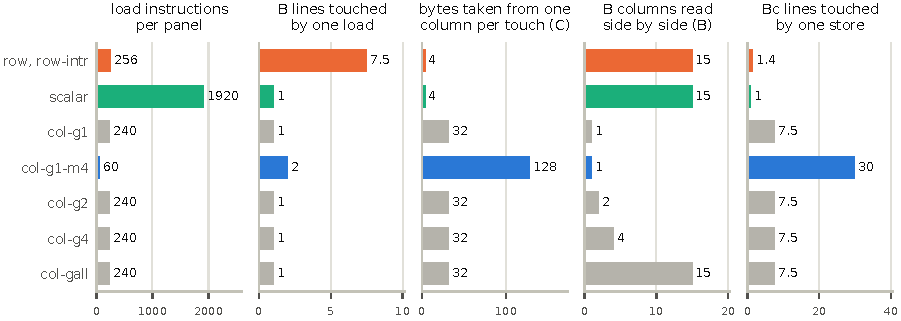
\includegraphics[width=\textwidth]{fig_counts.pdf}
\figcap{One full B panel on the default tile (B3, NR\,=\,15, kc\,=\,128, ldb\,=\,384), counted by replaying the loop nests of the
packers (\texttt{issue-54-figs/make\_figs.py}, \texttt{panel\_instructions}), with 64 B lines and line-aligned B and Bc. Not measured on
the board. Orange: the current order; blue: the fix; green: scalar.}
\label{fig:counts}
\end{figure}

\section{Results: B3 and B3\_K256}
Each cell is GOPs by mean time / GOPs by median rep / slow \%. Three tiles are pinned (16$\times$6, 16$\times$8, 16$\times$15), each on B3
(K=384) and B3\_K256. S1 is series 1, S2 is series 2. \texttt{row}, \texttt{col-g1-m4} and \texttt{col-gall} ran in both;
\texttt{row-intr}, \texttt{scalar} and \texttt{col-g1} in S1 only; \texttt{col-g2} and \texttt{col-g4} in S2 only. Red bold: bad cells (any slow reps, or steadily slow).
Figure~\ref{fig:headline}(a) shows the current packer, \texttt{scalar} and the fix side by side; Figure~\ref{fig:heatmap} shows every cell.

\begin{figure}[!htb]
\centering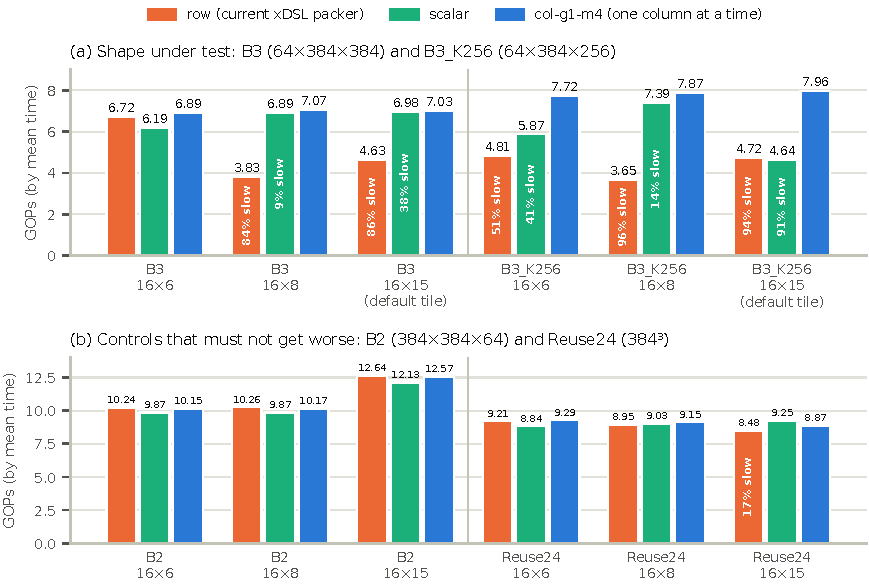
\includegraphics[width=0.9\textwidth]{fig_headline.pdf}
\figcap{Series 1 on \texttt{jbpi2}: \texttt{row}, \texttt{scalar} and \texttt{col-g1-m4} ran in the same night. Bar height is GOPs by mean
time over 3 launches; the white label inside a bar is its slow-rep share. Uninstrumented (\texttt{INSTRUMENTED=0}), reference protocol
\texttt{-{}-tmin 10}, core 4, \texttt{-{}-no-nc-overrides}. Source: \texttt{report\_series1\_jbpi2.md}, section 1.}
\label{fig:headline}
\end{figure}

\begin{figure}[!htb]
\centering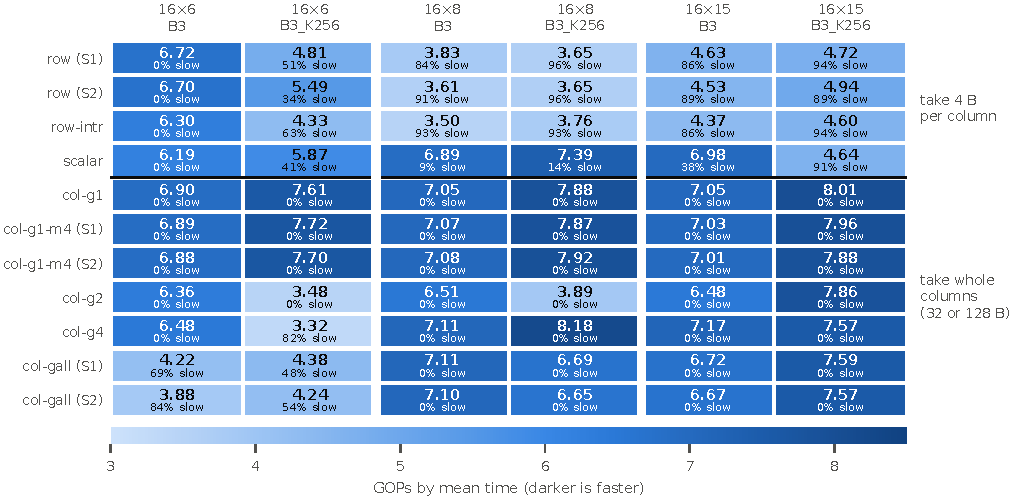
\includegraphics[width=0.9\textwidth]{fig_heatmap.pdf}
\figcap{Every GEMM cell of Tables 1 and 2: GOPs by mean time (bold) and slow-rep share. Darker is faster. Above the black line, the
orders that take 4 B per column; below it, the orders that take whole columns. A light cell with ``0\% slow'' (\texttt{col-g2} at
K\,=\,256) is the steadily slow state of \S\ref{sec:insight}. Same build, protocol and board as Figure~\ref{fig:headline}; sources: both
series reports, section 1.}
\label{fig:heatmap}
\end{figure}

\paragraph{Readers that take 4 bytes per column.}
\begin{center}\footnotesize\setlength{\tabcolsep}{2.8pt}
\begin{tabular}{@{}lcccccc@{}}
\toprule
 & \multicolumn{2}{c}{16$\times$6} & \multicolumn{2}{c}{16$\times$8} & \multicolumn{2}{c}{16$\times$15} \\
\cmidrule(lr){2-3}\cmidrule(lr){4-5}\cmidrule(lr){6-7}
variant & B3 & B3\_K256 & B3 & B3\_K256 & B3 & B3\_K256 \\
\midrule
\texttt{row} (S1) & \good{6.72/6.73/0} & \bad{4.81/5.33/51} & \bad{3.83/3.65/84} & \bad{3.65/3.55/96} & \bad{4.63/4.28/86} & \bad{4.72/4.56/94} \\
\texttt{row} (S2) & \good{6.70/6.71/0} & \bad{5.49/6.74/34} & \bad{3.61/3.34/91} & \bad{3.65/3.56/96} & \bad{4.53/4.28/89} & \bad{4.94/4.67/89} \\
\texttt{row-intr} & \good{6.30/6.33/0} & \bad{4.33/4.42/63} & \bad{3.50/3.30/93} & \bad{3.76/3.63/93} & \bad{4.37/4.18/86} & \bad{4.60/4.46/94} \\
\texttt{scalar} & \good{6.19/6.19/0} & \bad{5.87/6.47/41} & \bad{6.89/7.45/9} & \bad{7.39/7.91/14} & \bad{6.98/7.81/38} & \bad{4.64/4.42/91} \\
\bottomrule
\end{tabular}
\end{center}
{\footnotesize Table 1. Uninstrumented (INSTRUMENTED=0), reference protocol \texttt{-{}-tmin 10}, core 4, \texttt{-{}-no-nc-overrides}, 3 launches, board \texttt{jbpi2}.
Source: \texttt{report\_series1\_jbpi2.md} and \texttt{report\_series2\_jbpi2.md}, section 1.}

\paragraph{Readers that take whole columns.}
\begin{center}\footnotesize\setlength{\tabcolsep}{2.8pt}
\begin{tabular}{@{}lcccccc@{}}
\toprule
 & \multicolumn{2}{c}{16$\times$6} & \multicolumn{2}{c}{16$\times$8} & \multicolumn{2}{c}{16$\times$15} \\
\cmidrule(lr){2-3}\cmidrule(lr){4-5}\cmidrule(lr){6-7}
variant & B3 & B3\_K256 & B3 & B3\_K256 & B3 & B3\_K256 \\
\midrule
\texttt{col-g1} (S1) & \good{6.90/6.95/0} & \good{7.61/7.58/0} & \good{7.05/7.09/0} & \good{7.88/7.90/0} & \good{7.05/7.05/0} & \good{8.01/8.02/0} \\
\texttt{col-g1-m4} (S1) & \good{6.89/6.94/0} & \good{7.72/7.66/0} & \good{7.07/7.11/0} & \good{7.87/7.90/0} & \good{7.03/7.02/0} & \good{7.96/8.01/0} \\
\texttt{col-g1-m4} (S2) & \good{6.88/6.93/0} & \good{7.70/7.65/0} & \good{7.08/7.11/0} & \good{7.92/7.94/0} & \good{7.01/7.00/0} & \good{7.88/7.88/0} \\
\texttt{col-g2} (S2) & 6.36/6.39/0 & \bad{3.48/3.47/0} & 6.51/6.55/0 & \bad{3.89/3.89/0} & 6.48/6.48/0 & 7.86/7.91/0 \\
\texttt{col-g4} (S2) & 6.48/6.53/0 & \bad{3.32/3.01/82} & 7.11/7.13/0 & 8.18/8.21/0 & 7.17/7.17/0 & 7.57/7.59/0 \\
\texttt{col-gall} (S1) & \bad{4.22/4.50/69} & \bad{4.38/4.59/48} & 7.11/7.12/0 & 6.69/6.69/0 & 6.72/6.72/0 & 7.59/7.60/0 \\
\texttt{col-gall} (S2) & \bad{3.88/3.77/84} & \bad{4.24/4.47/54} & 7.10/7.11/0 & 6.65/6.66/0 & 6.67/6.67/0 & 7.57/7.58/0 \\
\bottomrule
\end{tabular}
\end{center}
{\footnotesize Table 2. Uninstrumented (INSTRUMENTED=0), reference protocol \texttt{-{}-tmin 10}, core 4, \texttt{-{}-no-nc-overrides}, 3 launches, board \texttt{jbpi2}.
Source: the same two reports, section 1. Green: no slow rep and in step with the other column readers.}

The two \texttt{col-g1} readers have no slow rep in any of their 18 cells, and the S1 and S2 cells of \texttt{col-g1-m4} agree to within
0.08 GOPs. The two \texttt{col-g2} cells at K=256 on 16$\times$6 and 16$\times$8 have no slow rep either, yet they run at
3.48 and 3.89 GOPs, against 7.70 and 7.92 for \texttt{col-g1-m4} (details in \S\ref{sec:insight}).

\emph{Cross-check on \texttt{jbpi}} (series 1 only): every GEMM cell falls in the same class, slow or steady. Steady \texttt{col-g1} and
\texttt{col-g1-m4} cells are within 0.15 GOPs of \texttt{jbpi2}, and cells in the slow state move by up to 0.43 GOPs.

\clearpage
\section{Results: the pack-only loop}
\label{sec:packonly}
This loop runs the B packer alone, with no compute between packs and one clock read per rep. Each cell is slow-rep share (\%) /
mean time of the fast reps (ms). When a packer is mostly slow, its ``fast'' mean is taken over few reps.

\begin{center}\footnotesize\setlength{\tabcolsep}{4pt}
\begin{tabular}{@{}lcccc@{}}
\toprule
 & \multicolumn{2}{c}{16$\times$15} & \multicolumn{2}{c}{16$\times$8} \\
\cmidrule(lr){2-3}\cmidrule(lr){4-5}
variant & B3 & B3\_K256 & B3 & B3\_K256 \\
\midrule
\texttt{row-intr} (S1) & \bad{91} / 0.6443 & \bad{33} / 0.3779 & \bad{91} / 0.8762 & 0 / 0.2185 \\
\texttt{scalar} (S1) & \bad{84} / 0.6571 & \bad{95} / 0.4179 & 5 / 0.6393 & 0 / 0.3776 \\
\texttt{col-g1} (S1) & 0 / 0.8907 & 0 / 0.4121 & 6 / 0.6086 & 7 / 0.2892 \\
\texttt{col-g1-m4} (S1) & 0 / 0.8218 & 0 / 0.3638 & 6 / 0.5598 & 5 / 0.2459 \\
\texttt{col-g1-m4} (S2) & 0 / 0.8525 & 0 / 0.3711 & 6 / 0.5599 & 4 / 0.2518 \\
\texttt{col-g2} (S2) & 0 / 1.1542 & 0 / 0.4821 & 0 / 0.8949 & 0 / 0.6583 \\
\texttt{col-g4} (S2) & 0 / 1.0525 & 0 / 0.5111 & 0 / 0.8039 & 0 / 0.3488 \\
\texttt{col-gall} (S1) & 0 / 1.4031 & 0 / 0.6554 & 0 / 1.0775 & 0 / 0.3307 \\
\texttt{col-gall} (S2) & 0 / 1.3852 & 0 / 0.6840 & 0 / 1.0925 & 0 / 0.3265 \\
\bottomrule
\end{tabular}
\end{center}
{\footnotesize Table 3. Uninstrumented (INSTRUMENTED=0), reference protocol \texttt{-{}-tmin 10}, core 4, \texttt{-{}-no-nc-overrides}, 3 launches, board \texttt{jbpi2}.
Source: \texttt{report\_series1\_jbpi2.md} and \texttt{report\_series2\_jbpi2.md}, section 2. \texttt{row} and 16$\times$6 are not in this loop.}

With 4-byte reads, the packer alone shows two speeds: \texttt{row-intr} is 91\% slow at 16$\times$15 and at 16$\times$8 on B3, and \texttt{scalar} is
84--95\% slow at 16$\times$15. The column readers stay at 0--7\%. The 4--7\% slow reps of \texttt{col-g1} and \texttt{col-g1-m4} at 16$\times$8 are
isolated reps (for example 0.5598 ms fast against 0.7851 ms slow for \texttt{col-g1-m4} at B3), and they do not show in the GEMM cells.

\paragraph{The two speeds, rep by rep (Figure~\ref{fig:reps}).} With the current order, the GEMM is fast for its first 18 reps, becomes slow
at 0.05 s and stays in a band near 4.3 GOPs (median of the slow reps 4.33), with short returns to the fast speed; the B packer alone does the same, from about 0.6 ms to about 1.3 ms per rep.
With \texttt{col-g1-m4}, both stay in one band for the whole run.

\paragraph{Average cost per pack (Figure~\ref{fig:packcost}).} Averaged over all reps, slow ones included, a pack of B3 takes 0.822 ms
with \texttt{col-g1-m4} against 1.155 ms with \texttt{row-intr} at 16$\times$15, and 0.574 ms against 1.147 ms at 16$\times$8. A fast
\texttt{row-intr} rep is cheaper (the black tick), but it is rare. \texttt{row} itself is not in this loop, so these are against its
C-intrinsics copy.

\begin{figure}[!htb]
\centering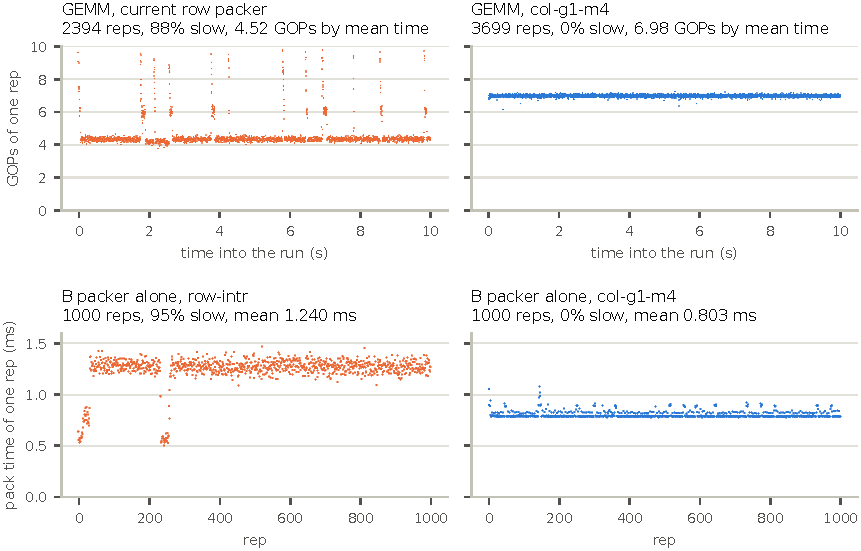
\includegraphics[width=\textwidth]{fig_reps.pdf}
\figcap{Every rep of one launch, B3 on the default 16$\times$15 tile. Top: the full GEMM, series 2 launch 1 (\texttt{row}:
\texttt{run\_2026-10-23\_101023}; \texttt{col-g1-m4}: \texttt{run\_2026-10-23\_103733}), one dot per rep against the time into the
10 s run. Bottom: the B packer alone, series 1 launch 1 (\texttt{packonly\_jbpi2\_L1\_*\_B3\_16x15.txt}), 1000 reps after 5 warm-up reps.
Slow shares use the same split as the series reports. Single launches, so the shares differ a little from the 3-launch
averages in Tables 1 and 3. Uninstrumented, reference protocol \texttt{-{}-tmin 10}, core 4, \texttt{-{}-no-nc-overrides}, \texttt{jbpi2}.}
\label{fig:reps}
\end{figure}

\begin{figure}[!htb]
\centering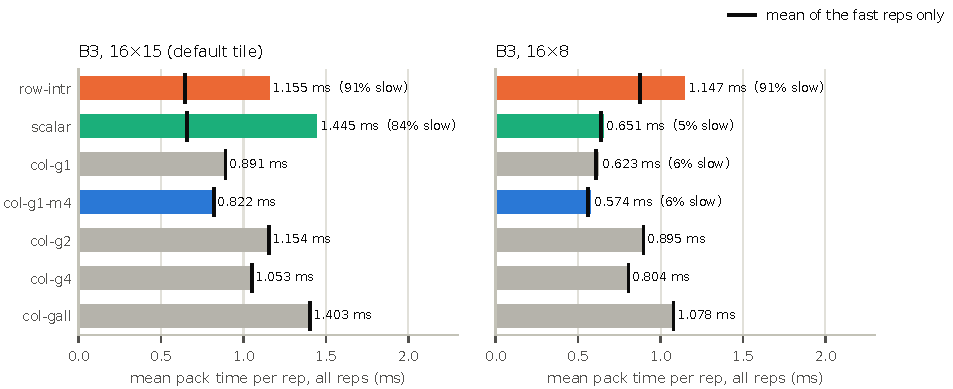
\includegraphics[width=\textwidth]{fig_pack_cost.pdf}
\figcap{The B packer alone on B3. Bar: mean time per rep over all reps, the average of 3 launches; black tick: the mean of the fast
reps only (the number in Table 3). \texttt{col-g2} and \texttt{col-g4} are from series 2, the rest from series 1. Uninstrumented,
core 4, \texttt{jbpi2}; source: the \texttt{packonly\_jbpi2\_L*} files of both series.}
\label{fig:packcost}
\end{figure}

\section{Results: the controls B2 and Reuse24}
Mean GOPs; the slow-rep share in brackets when it is not zero (series 1 shown in Figure~\ref{fig:headline}(b)). B2 uses kc$=$64; Reuse24 uses the same kc as B3 at each tile (256, 256, 128).

\begin{center}\footnotesize\setlength{\tabcolsep}{4pt}
\begin{tabular}{@{}lcccccc@{}}
\toprule
 & \multicolumn{3}{c}{B2} & \multicolumn{3}{c}{Reuse24} \\
\cmidrule(lr){2-4}\cmidrule(lr){5-7}
variant & 16$\times$6 & 16$\times$8 & 16$\times$15 & 16$\times$6 & 16$\times$8 & 16$\times$15 \\
\midrule
\texttt{row} (S1) & 10.24 & 10.26 & 12.64 & 9.21 & 8.95 & \bad{8.48 (17)} \\
\texttt{row} (S2) & 10.26 & 10.24 & 12.47 & 9.21 & 8.96 & \bad{8.68 (14)} \\
\texttt{row-intr} & 10.05 & 10.18 & 12.33 & 8.89 & \bad{7.07 (73)} & \bad{7.55 (53)} \\
\texttt{scalar} & 9.87 & 9.87 & 12.13 & 8.84 & 9.03 & 9.25 \\
\texttt{col-g1} & 10.13 & 10.19 & 12.43 & 9.28 & 9.17 & 8.86 \\
\texttt{col-g1-m4} (S1) & 10.15 & 10.17 & 12.57 & 9.29 & 9.15 & 8.87 \\
\texttt{col-g1-m4} (S2) & 10.24 & 10.24 & 12.46 & 9.27 & 9.15 & 8.88 \\
\texttt{col-g2} (S2) & 10.17 & 10.13 & 12.49 & 9.17 & 9.09 & 8.71 \\
\texttt{col-g4} (S2) & 10.24 & 10.15 & 12.40 & 9.16 & 9.13 & 8.93 \\
\texttt{col-gall} (S1) & 10.19 & 10.17 & 12.38 & 9.10 & 8.99 & 8.74 \\
\texttt{col-gall} (S2) & 10.22 & 10.21 & 12.43 & 9.08 & 8.99 & 8.73 \\
\bottomrule
\end{tabular}
\end{center}
{\footnotesize Table 4. Uninstrumented (INSTRUMENTED=0), reference protocol \texttt{-{}-tmin 10}, core 4, \texttt{-{}-no-nc-overrides}, 3 launches, board \texttt{jbpi2}.
Source: the two reports, section 1 (B2 and R24 blocks).}

On B2 the column readers are within 0.26 GOPs of \texttt{row} (largest gap 12.64 against 12.38, \texttt{col-gall} S1, at 16$\times$15;
\texttt{col-g1-m4} at most 0.09); \texttt{scalar} is lower
by 0.37 to 0.51. Reuse24 becomes slow only with \texttt{row} (16$\times$15: 17\% in S1, 14\% in S2) and with \texttt{row-intr}
(16$\times$8: 73\%; 16$\times$15: 53\%). No column reader becomes slow on either control.

\section{What it means for the design}
\label{sec:insight}
\begin{enumerate}
  \item \textbf{A read pattern sets off the slow state; the vector unit and the number of streams do not.} What \texttt{row},
  \texttt{row-intr} and \texttt{scalar} share is that they take 4 B from each of NR columns that lie 1536 B (B3) or 1024 B (B3\_K256) apart, then move to the next k.
  Scalar loads do it too: pack-only is 84--95\% slow at 16$\times$15, and the full GEMM is 91\% slow at 16$\times$15 on B3\_K256. So the
  \iss{53} finding that ``scalar is steadier'' depends on the tile.
  \item \textbf{The B packer alone can set the state off.} In the pack-only loop, with no compute, \texttt{row-intr} is 91\% slow at
  16$\times$15 and at 16$\times$8 on B3. So the next step belongs in the packer, not in the order of pack and compute.
  \item \textbf{Reading a column 32 B or 128 B at a time removes this trigger.} \key{One column at a time is the only order that is safe on
  every cell we ran.}
  \item \textbf{Grouping columns brings back bad cells that follow tile and K, not group size.} \texttt{col-g2} is bad at K=256
  (16$\times$8 and 16$\times$6), \texttt{col-g4} is bad at 16$\times$6 on K=256, and \texttt{col-gall} is bad at 16$\times$6 at both K.
  This looks like placement (where the active lines land in the cache), which fits \iss{49}, and not a limit on the number of streams.
  The idea in \iss{44} is right in its effect (one column at a time), but for a different reason.
  \item \textbf{A third state: steadily slow.} \texttt{col-g2} at 16$\times$8 on B3\_K256 runs at 3.89 GOPs with a launch spread of 0.02
  (3.88--3.90) and no two-speed split. Its pack alone is a uniform 0.6448 ms (median), against 0.2500 ms for \texttt{col-g1-m4}.
  A tool that splits reps into fast and slow reports this cell as 0\% slow. Read the GOPs together with the slow share.
  \item \textbf{Cost.} In a fast rep, a one-column pack costs a little more than \texttt{row-intr}'s: at 16$\times$15 on B3 the pack-only
  fast mean is 0.8218 ms for \texttt{col-g1-m4} against 0.6443 ms. But it never becomes slow, while \texttt{row-intr} spends 91\% of its
  reps at 1.1994 ms.
  \item \textbf{The flaw is in the standard packing method, not only in this design: the reference has it too.} The reference design
  (\texttt{gemm\_blis\_family} in \texttt{RVV\_ukernels\_benchmark}) packs B in the same order: the code read of \iss{52} found that its B
  packer visits the same addresses in the same order as ours, 4 B from each column across a row, only with one scalar load per
  element. And it falls into the same slow state on B3\_K256 (\iss{46}, below). On plain B3 the reference was much steadier than ours in \iss{46}, but not in the new run below (81\% slow at 16$\times$14);
  why is not settled. The likely reasons are its tile (16$\times$14 against our 16$\times$15) and where its buffers land: the
  per-rep timing patch moved its B3 speed in opposite directions on the two boards. Since it reads B the same way, the one-column
  packer should help the reference too, and the new run below confirms it (16$\times$14: 4.49 $\to$ 7.14 GOPs). The exact code of both packers is in Appendix~C.

  Figure~\ref{fig:refvsours} shows the reads of the two packers and of the fix, on the matrix and on the memory addresses.

  \begin{figure}[!htb]
  \centering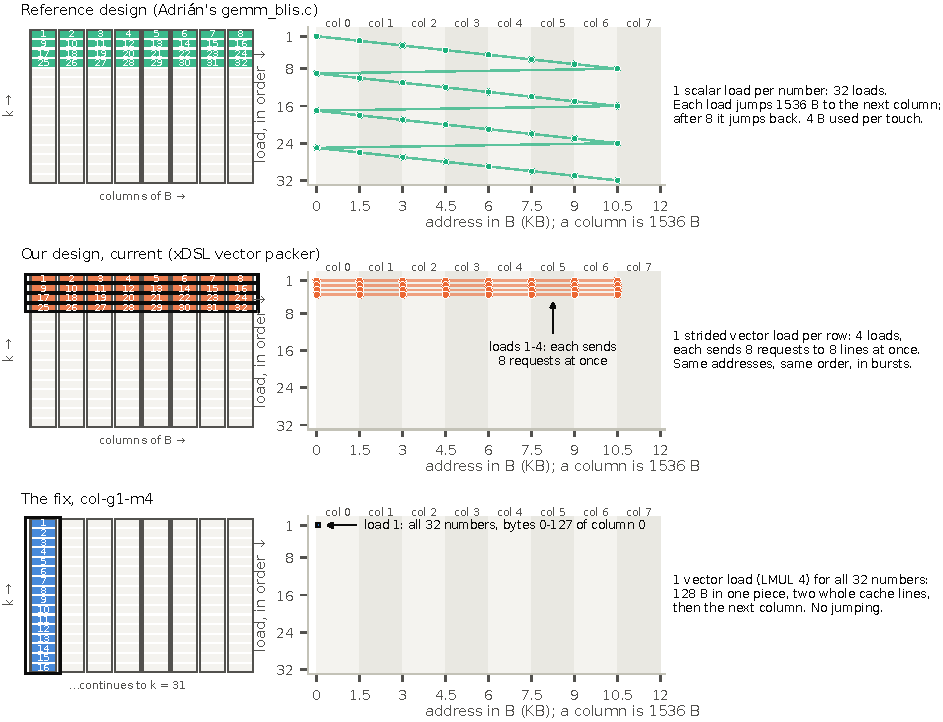
\includegraphics[width=\textwidth]{fig_ref_vs_ours.pdf}
  \figcap{The first 32 numbers each packer reads from B3's B (K\,=\,384, so the columns are 1536 B apart). Left: on the matrix, numbered
  in read order; one cache line is one outlined column of 16 numbers. Right: the same reads on the memory addresses of B, one row per load
  instruction. The reference (\texttt{pack\_CB} in \texttt{gemm\_blis.c}) and the current xDSL packer read the same numbers in the
  same order: 4 B from column 0, then 1536 B further for column 1, and so on, back to column 0 after 8. The reference issues one load per
  number; ours issues one strided vector load per row, so the same 8 scattered requests leave at once. The fix reads 32 numbers down one
  column with one load. Drawn from the code, NR\,=\,8; at NR\,=\,15 the jump-back comes after 15 columns.}
  \label{fig:refvsours}
  \end{figure}

  \begin{center}\footnotesize\setlength{\tabcolsep}{5pt}
  \begin{tabular}{@{}lcc@{}}
  \toprule
  slow reps (\texttt{jbpi} / \texttt{jbpi2}) & ours, 16$\times$15, vector packer & reference, 16$\times$14 \\
  \midrule
  B3\_K256 & \bad{94\% / 88\%} & \bad{80\% / 60\%} \\
  B3 & \bad{87--89\%}, 4.4--4.5 GOPs & \bad{22\%} / 0\%, 7.1--7.6 GOPs \\
  \bottomrule
  \end{tabular}
  \end{center}
  {\footnotesize Table 5. From \iss{46} (2026-09-29, an older series than the rest of this brief, run in quiet windows on both boards):
  uninstrumented, reference protocol \texttt{-{}-tmin 10}, core 4; the reference driver patched only to record the time of each rep.
  Not the same night as Tables 1--4, so compare within this table only.}

  \textbf{New run: the reference design with our fix (2026-10-29).} Adrián's reference design was run again on B3, as it is and
  with its \texttt{pack\_CB} replaced by our one-column packer (\texttt{ref\_baseline/ref\_pack\_fix.py}, a staged copy; nothing else
  changed; the result check passes with error 0 on both tiles). At 16$\times$14 the reference as it is was \bad{81\%} slow, 4.49 GOPs
  (4.39--4.60 over 3 launches); \key{with the fix it had no slow rep, 7.14 GOPs (7.11--7.18), +59\%.} At 16$\times$16, a kernel that is
  slower for its own reasons (it needs 34 vector registers, \iss{46}), the fix moves it from 4.20 to 4.41 GOPs and from 22\% to 0\%
  slow (Figures~\ref{fig:refcompare} and~\ref{fig:refreps}). This differs from \iss{46}, where the reference's B3 at 16$\times$14 was
  0--22\% slow. That run timed four shapes in one binary and this one times B3 alone, and \iss{46} found that the reference's B3
  speed moves with where its buffers land; so the reference is not reliably steadier on B3 than our design. \key{The fix removes the slow
  state in both designs.}

  \begin{figure}[!htb]
  \centering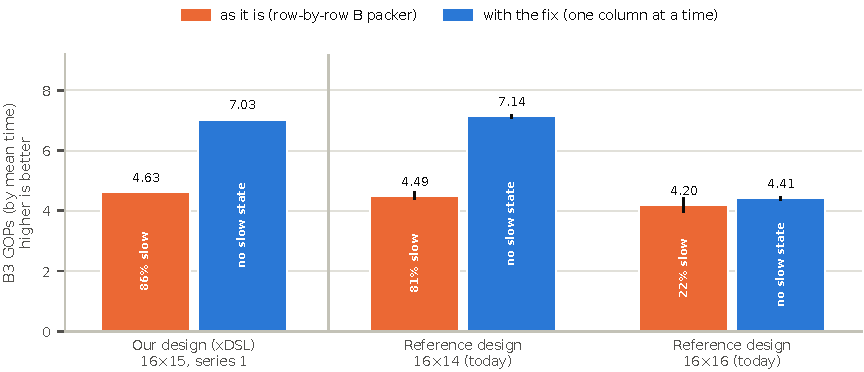
\includegraphics[width=0.92\textwidth]{fig_ref_compare.pdf}
  \figcap{B3 with and without the fix, in our design and in the reference design. Bar: GOPs by mean time, average of 3 launches; thin
  line: lowest to highest launch; text in the bar: share of slow reps. Our design: series 1 (2026-10-22, Table 1). Reference design:
  2026-10-29, the reference's own driver, packers and LDX \texttt{macc} kernels, with the per-rep record; the reference has no
  16$\times$15 kernel, so its neighbours 16$\times$14 and 16$\times$16 run. Different nights: compare within each design, not across.
  All uninstrumented, reference protocol \texttt{-{}-tmin 10}, core 4, board \texttt{jbpi2}, launch order A B, B A, A B; the board
  was 98.6--99.5\% idle with no other user before and after every run. Run folders: series \texttt{logs/issue54\_ref\_2026-10-29\_123319} (\texttt{runs.tsv}; reference
\texttt{refbase\_2026-10-29\_123934}, \texttt{\_125611}, \texttt{\_130140}; with the fix \texttt{refbase\_2026-10-29\_124512},
\texttt{\_125042}, \texttt{\_130709}).}
  \label{fig:refcompare}
  \end{figure}

  \begin{figure}[!htb]
  \centering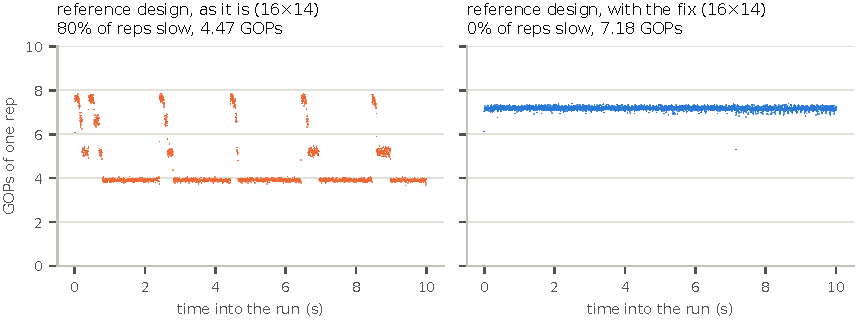
\includegraphics[width=\textwidth]{fig_ref_reps.pdf}
  \figcap{Every rep of launch 1, B3, the reference design at 16$\times$14: as it is (left, \texttt{refbase\_2026-10-29\_123934}) and with
  our fix in its packer (right, \texttt{refbase\_2026-10-29\_124512}). The same two speeds as in our design (Figure~\ref{fig:reps}); with
  the fix, one speed. Same build, protocol, core and board as Figure~\ref{fig:refcompare}.}
  \label{fig:refreps}
  \end{figure}

  \item \textbf{Our vector packer makes the slow state more frequent in most cells, but it does not cause it.} Same night, same board
  (Table 1, series 1), share of slow reps, vector \texttt{row} against \texttt{scalar}: 84\% against 9\% at 16$\times$8 B3, 96\% against
  14\% at 16$\times$8 B3\_K256, 86\% against 38\% at 16$\times$15 B3, 51\% against 41\% at 16$\times$6 B3\_K256. But at 16$\times$15
  B3\_K256 both are slow (94\% and 91\%), at 16$\times$6 B3 neither is, and in the pack-only loop the order is reversed at 16$\times$15
  B3\_K256 (\texttt{row-intr} 33\%, \texttt{scalar} 95\%, Table 3). When neither is slow, the vector packer is the faster one (6.72
  against 6.19 GOPs at 16$\times$6 B3). A likely reason, not measured: one strided vector load sends 8 requests to 8 different lines at
  once, where the scalar packer sends the same 8 one by one, so the bad pattern arrives in bursts. So the cause is the read pattern,
  which vector, scalar and the reference share. The vector packer makes it worse in most cells. Going back to scalar does not fix it,
  and vectors are not the problem: the fix uses even wider vector loads (32 numbers instead of 8), pointed down a column instead of
  across a row.
  \item \textbf{What the reference developer says, and what the code and data show.} The reference developer's view (2026-10-29):
  the packing and unpacking themselves have no obvious flaw; the address jumping when B is read is harmless in their scalar packer,
  which reads one element at a time, and becomes a problem when that loop is widened into vector code. The machine code agrees
  (Appendix~C.6): the reference's packer, built with \texttt{-O3 -march=rv64gcvzfh}, has no vector instruction at all, one
  \texttt{flw}/\texttt{fsw} pair per number, 1536 B apart; ours turns the same loop into \texttt{vlse32.v} gathers that send 8 (then 7)
  requests to as many columns at once. The data mostly agrees too:
  \begin{itemize}
    \item On B3 the scalar reference is 0--22\% slow, ours 87--89\% (Table 5); our own scalar packer is 9--14\% slow at 16$\times$8
    against 84--96\% for our vector packer, and 38\% against 86\% at 16$\times$15 on B3 (Table 1). So, in these runs, widening the
    loop makes our design fall into the slow state far more often.
    \item But the new run of 2026-10-29 (Figure~\ref{fig:refcompare}) found the scalar reference 81\% slow on B3 at 16$\times$14 as
    well, and our fix removed it there too (4.49 $\to$ 7.14 GOPs). So one number per load does not keep B3 steady in every run.
  \end{itemize}
  With one limit: the row-by-row order is not entirely free of the problem with scalar loads either. The reference is still 60--80\%
  slow on B3\_K256 (Table 5), our scalar packer is 91\% slow at 16$\times$15 on B3\_K256 (Table 1), and alone it is 84--95\% slow at
  16$\times$15 (Table 3). So the precise statement is: the packing is correct and its row-by-row order is mostly harmless with scalar
  loads; widening it into strided vector gathers makes the slow state much more frequent; and on K\,=\,256 the order costs even with
  scalar loads. The fix keeps the vector width and changes the direction of the reads, so it avoids both (Tables 1--2). B itself is
  only packed, never unpacked, in the GEMM, so unpacking plays no part here.
\end{enumerate}

\section{Is the fix worth it? Compared with the simpler choices}
\label{sec:worth}
Two simpler choices exist and need no new code: turn on the scalar B packer the generator already has (its switch is
\texttt{use\_scalar\_pack}), or choose a smaller tile. Table~6 puts the current packer, the scalar packer and the fix side by side on every layer and tile, from the same
night (series 1).

\begin{center}\footnotesize\setlength{\tabcolsep}{4pt}
\begin{tabular}{@{}llccccc@{}}
\toprule
layer & tile & current (vector) & scalar & the fix & fix vs current & fix vs scalar \\
\midrule
B3 & 16$\times$6 & 6.72 & 6.19 & 6.89 & +3\% & +11\% \\
B3 & 16$\times$8 & \bad{3.83 (84\%)} & \bad{6.89 (9\%)} & 7.07 & +85\% & +3\% \\
B3 & 16$\times$15 (default) & \bad{4.63 (86\%)} & \bad{6.98 (38\%)} & 7.03 & +52\% & +1\% \\
B3\_K256 & 16$\times$6 & \bad{4.81 (51\%)} & \bad{5.87 (41\%)} & 7.72 & +60\% & +32\% \\
B3\_K256 & 16$\times$8 & \bad{3.65 (96\%)} & \bad{7.39 (14\%)} & 7.87 & +116\% & +6\% \\
B3\_K256 & 16$\times$15 (default) & \bad{4.72 (94\%)} & \bad{4.64 (91\%)} & 7.96 & +69\% & +72\% \\
\midrule
B2 & 16$\times$6 & 10.24 & 9.87 & 10.15 & $-$1\% & +3\% \\
B2 & 16$\times$8 & 10.26 & 9.87 & 10.17 & $-$1\% & +3\% \\
B2 & 16$\times$15 (default) & 12.64 & 12.13 & 12.57 & $-$1\% & +4\% \\
Reuse24 & 16$\times$6 & 9.21 & 8.84 & 9.29 & +1\% & +5\% \\
Reuse24 & 16$\times$8 & 8.95 & 9.03 & 9.15 & +2\% & +1\% \\
Reuse24 & 16$\times$15 (default) & \bad{8.48 (17\%)} & 9.25 & 8.87 & +5\% & $-$4\% \\
\bottomrule
\end{tabular}
\end{center}
{\footnotesize Table 6. GOPs by mean time, 3 launches; in brackets the slow-rep share when it is not zero. Series 1, the same night for all
three packers; uninstrumented (\texttt{INSTRUMENTED=0}), reference protocol \texttt{-{}-tmin 10}, core 4, \texttt{-{}-no-nc-overrides},
board \texttt{jbpi2}. Source: \texttt{report\_series1\_jbpi2.md}, section 1. The fix's 1\% losses on B2 are inside the run-to-run spread.}

\paragraph{Is the improvement large?} Against the current packer, yes, but only on the B3 family: \key{+52\% on B3 and +69\%
on B3\_K256} on the default tile, up to +116\% at 16$\times$8. On the large layers (B2, Reuse24) it changes almost nothing ($-$1\% to
+5\%). So it is a large improvement for one class of layers (small M, large K; \iss{35} found the slow state up to M\,=\,512 on the default
tile), not a speed-up of the whole design.

\paragraph{Why not simply keep a scalar packer?} On plain B3 at the default tile, scalar is almost as good (6.98 against 7.03 GOPs),
needs no new code, and is how the reference packs. But it is not enough on its own:
\begin{itemize}
  \item it still falls into the slow state on B3\_K256 at the default tile (91\% slow, 4.64 GOPs, against 7.96 for the fix), and on
  16$\times$6 (41\%);
  \item when nothing is slow it is slower: $-$3 to $-$4\% on B2, the largest layer (12.13 against 12.64 at 16$\times$15), and
  $-$8\% on B3 at 16$\times$6 (6.19 against 6.72);
  \item it is better than the fix in only one cell, Reuse24 at 16$\times$15 (9.25 against 8.87).
\end{itemize}
So scalar packing trades a 3--4\% loss on the large layers for a fix that holds on B3 but not on B3\_K256. \key{The fix is the only one of
the three that is never slow and never clearly slower}: best or within 1\% in 11 of the 12 cells.

\paragraph{Why not a smaller tile?} 16$\times$6 keeps B3 steady with the current packer (6.72 GOPs), but not B3\_K256 (51\% slow), and it
costs 19\% on B2 (10.24 against 12.64). It is not a fix.

\paragraph{Is it over-engineering?} The change itself is small: 16 lines of C intrinsics (Figure~\ref{fig:codediff}), the same
instructions the packer already uses, turned to read down the columns. The real cost is the xDSL port: the dialect has no fp32 strided
store yet (\iss{44}). Whether that cost is worth paying depends on one thing we have not measured: \textbf{how much of a real model's
time is spent in layers like B3} (small M, K of 256 or more). If those layers are rare, the scalar switch, or the current packer, is
good enough; if they are common, the fix is the only choice here that removes the slow state everywhere.

\paragraph{Is packing itself needed?} This work does not test a GEMM without packing; both designs pack, as BLIS does, so that the
microkernel reads Bc in order. The question here is only which packer, not whether to pack.

\paragraph{Recommendation.} Before the xDSL port, take the layer list of the target models and count the time in small-M,
large-K layers (desk work, from the existing per-layer runs). \key{Port the fix if that share is significant;} otherwise switch the scalar
packer on for those layers only, and accept the B3\_K256 gap.

\section{Caveats}
\begin{itemize}
  \item The control holds only in part. On the 16$\times$8 and 16$\times$15 cells, \texttt{row-intr} is within 0.35 GOPs of \texttt{row}
  with the same kind of slow share. But it is lower on 16$\times$6 B3 (6.30 against 6.72, S1), and 16$\times$6 B3\_K256 differs more
  (4.33 against 4.81, 63\% against 51\% slow). It also becomes slow on Reuse24 where \texttt{row} does not (16$\times$8). The C-intrinsics
  copy is not identical to the xDSL packer. The gains of \texttt{col-g1} hold against both.
  \item \texttt{col-g1-m4} exists only as C intrinsics. Using it in the generator needs an xDSL port. That is out of scope here, because the
  dialect has no fp32 strided store (\iss{44}).
  \item Only B3-family shapes plus two controls, three pinned tiles and one board model. No counters were read in these runs
  (uninstrumented), so the prefetcher explanation is inferred from \iss{50}, not measured here.
  \item \textcolor{red}{RED NOTE, \texttt{jbpi} (cross-check board only).} One GEMM run was discarded for another user's compile, and one pack-only
  run because overall idle fell to 84.8\%, under the 85\% gate; both were redone. Core 3 was at 72\% during one 16$\times$15 binary of \texttt{run\_2026-10-22\_214815} (\texttt{col-g1-m4}, launch 2),
  and root \texttt{bluetoothd} used 20--99\% of one core in the live \texttt{top} readings (median 55\%). \texttt{jbpi} numbers are used only as a cross-check; every number in the
  tables above is from \texttt{jbpi2}.
  \item The slow share of \texttt{row} moves between nights on some cells (16$\times$6 B3\_K256: 51\% in S1, 34\% in S2).
\end{itemize}

\section{Next steps}
\begin{itemize}
  \item Port \texttt{col-g1-m4} to xDSL (new ticket; it needs a strided fp32 store, or the unit-stride load and strided store pair).
  \item One counter run (\iss{50} style) of \texttt{row} against \texttt{col-g1-m4} on B3 16$\times$15, to confirm the prefetcher explanation.
  \item Look at the bad cells of the grouped readers against the addresses of Bc and B (placement). This is desk work and needs no board time.
  \item Report-script fixes: flag cells that are uniformly slow; a false RED from the lifetime \%CPU in \texttt{ps}; mid-run load taken
  from the per-core monitor.
\end{itemize}

\section*{Appendix A: sources}
\raggedright\emergencystretch=3em
\begin{itemize}
  \item Branch \texttt{issue55-pack-b-variants}: \texttt{5338a3b8} (variants), \texttt{c85f7f7d} (switch), \texttt{d0de1b0f} (pack-only loop, series
  and report scripts), \texttt{383c886c} (series 1 logs), \texttt{bf6f2366} (series 2 logs).
  \item Logs, under \path{tests/pure_xdsl_blis_rvv/}: \path{logs/issue55_2026-10-22_194043/report_series1_jbpi2.md};
  \path{logs/issue55_jbpi/issue55_2026-10-22_194043/report_series1_jbpi.md} (cross-check);
  \path{logs/issue55_2026-10-23_100122/report_series2_jbpi2.md}.
  \item Reference design with and without the fix (2026-10-29): series \path{logs/issue54_ref_2026-10-29_123319} and its six
  \path{refbase_2026-10-29_*} run folders; code \path{ref_baseline/ref_pack_fix.py}, \path{run_issue54_ref.sh},
  \path{ref_baseline/cases_issue54_b3.tsv}.
  \item Figures: \path{.scratch/reports/issue-54-figs/make_figs.py} builds every figure from the logs above (run it from the
  repo root with the project venv). Figures~\ref{fig:units}--\ref{fig:counts} are drawn and counted from the code, not measured.
  \item Issues \iss{54} (question), \iss{55} (spec), \iss{48}, \iss{49}, \iss{50}, \iss{53}, \iss{44}.
\end{itemize}

\clearpage
\section*{Appendix B: the finding in three minutes}
\label{sec:short}
A short version for a presentation, in plain words. It compares only three packers: the reference design's, our current xDSL packer, and
the fix. Each step shows the figure to put on screen. All speeds are from the uninstrumented build, reference protocol, core 4,
board \texttt{jbpi2}.

\newcommand{\step}[3]{\par\noindent\begin{minipage}{\textwidth}\textbf{#1}\par\smallskip #2\par\smallskip
\ifdim #3pt>0pt {\centering\includegraphics[width=#3\textwidth]{\stepfig}\par}\fi\end{minipage}\par\bigskip}

\def\stepfig{fig_short_reps.pdf}
\step{1. The problem: the slow state.}{B3 is one layer of our GEMM. On the default tile it should run at about 7 GOPs, but it runs
at about 4.5. It is not slow all the time: it starts fast, and after 18 reps (0.05 s) it drops to a slow speed and mostly stays
there. We call this the \emph{slow state}. \key{About 9 reps out of 10 are slow.} Left: our current packer; right: the fix.}{0.9}

\def\stepfig{fig_ref_reps.pdf}
\step{1b. The same problem in the reference design (Figure~\ref{fig:refreps}).}{Adrián's reference design, run on the same board in
the same way (2026-10-29), shows the same two speeds on B3 at its nearest tile, 16$\times$14: fast for a moment, then about 3.9 GOPs,
81\% of reps slow. With our fix in its packer, \key{it stays at about 7.1--7.2 GOPs with no slow rep.} Left: the reference as it is; right:
the reference with the fix.}{0.9}

\step{2. What we saw before this work.}{%
\begin{itemize}
  \item In slow reps the hardware prefetcher works about half as well: it brings in half as many cache lines ahead of time (\iss{50}).
  \item The slow state depends on how B is packed, not on the compute part (\iss{48}).
  \item The packer run alone, with no compute, still becomes slow.
\end{itemize}
So the packer's memory reads are what set it off.}{0}

\def\stepfig{fig_ref_vs_ours.pdf}
\step{3. The reason: how the packer reads B (Figure~\ref{fig:refvsours}).}{B is stored column by column. The current packer reads
across a row: one load takes one number (4 bytes) from each of 8 columns that sit far apart in memory (8 numbers of 4 bytes, 32 bytes in
total). \key{So one load touches 8
different cache lines and uses only 4 bytes from each.} The prefetcher most likely cannot follow this pattern, so it stops helping,
and pack and compute both slow down. Top: the reference design reads B the same way, one number per load. Middle: our
current packer, the same reads sent 8 at a time. Bottom: the fix, 32 numbers from one place with one load.}{0.9}

\def\stepfig{fig_short_slow.pdf}
\step{4. The finding.}{The trigger is the read pattern: 4 bytes taken from each of many columns that sit far apart. \key{Reading B one
column at a time removes it:} the fix has no slow rep on any tile or K we tested, on both boards and on both nights. The figure shows
the share of slow reps, our current packer against the fix.}{0.85}

\def\stepfig{fig_ref_compare.pdf}
\step{5. Is it our design, or the packing method? (\S\ref{sec:insight}, Figure~\ref{fig:refcompare})}{%
\begin{itemize}
  \item \textbf{The reference design reads B the same way.} Its packer takes 4 B from each column across a row, like ours, but one
  number per load (scalar). It also becomes slow on B3\_K256: 80\% and 60\% of reps on the two boards, against 94\% and 88\% for ours.
  So the read order itself is a weakness of the standard packing method on this chip.
  \item \textbf{Measured today, with and without the fix, in both designs (figure below).} The reference at 16$\times$14 was 81\% slow
  on B3 (4.49 GOPs); with our fix in its packer it had no slow rep (7.14 GOPs, +59\%). Our design: 86\% slow, 4.63 GOPs; with the fix,
  7.03 GOPs. \key{The fix removes the slow state in both designs.}
  \item \textbf{Our design makes it much worse, by widening the loop into vector loads.} The reference developer's view: the packing
  itself has no flaw; jumping between columns is harmless when each load takes one number, and hurts when the loop is widened into
  vector loads that send 8 scattered requests at once. The machine code confirms the difference (Appendix~C.6): the reference packer
  has no vector instruction at all, ours gathers 8 numbers per instruction. An older run (\iss{46}) agreed: on B3 the reference was
  0--22\% slow, ours 87--89\%. But today's run found the reference 81\% slow on B3 as well, and it is 60--80\% slow on B3\_K256, so one
  number per load is not a full cure: the reference's B3 speed depends on the run (most likely on where its buffers land).
  \item \textbf{The answer is not to drop vectors, but to point them down the columns.} The fix is itself a vector packer, with wider
  loads.
  \item \textbf{The code} of the reference, our xDSL packer and the fix, and the machine code of all three, is in Appendix~C.
\end{itemize}
The figure: B3, each design as it is (orange) and with the fix (blue); our design from 2026-10-22, the reference from 2026-10-29,
so compare within each design.}{0.9}

\def\stepfig{fig_code_diff.pdf}
\step{6. The solution (Figure~\ref{fig:codediff}).}{%
\fcolorbox{blue!50!black}{blue!4}{\parbox{0.97\textwidth}{\textbf{The fix (\texttt{col-g1-m4}), in one sentence:} read B one column
at a time, 32 numbers per load, then write those numbers into their places in Bc.}}

\smallskip
\textbf{How it works, step by step.}
\begin{enumerate}
  \item Take one column of B. B is stored column by column, so its numbers sit next to each other in memory.
  \item Load 32 of them at once: 128 B, exactly two whole cache lines. Four vector registers are joined into one long register to hold
  them (LMUL\,=\,4, the ``m4''; here the 4 counts registers: 4 registers of 8 numbers = 32 numbers).
  \item Write the 32 numbers into Bc. In Bc they belong in one column of the panel, so this is a strided store (one number every
  NR$\times$4 B; here the 4 is bytes per number, so at NR\,=\,15 the numbers land 60 B apart, one per row of the panel).
  \item Go on down the column, then move to the next column.
\end{enumerate}
\textbf{Why it works.}
\begin{itemize}
  \item It reads memory in the order it is stored: whole cache lines from one place, not 4 B from 8 places far apart.
  \item Each cache line of B is touched once and fully used. The current packer visits each line 16 times and takes 4 B each time.
  \item Only one column is read at a time, so only one read stream is open.
  \item The jumping moves from the reads of B to the writes into Bc, which is the cheaper side to pay it on.
  \item Fewer instructions: 60 loads per panel instead of 256 (B3, default tile).
\end{itemize}
\textbf{What does not change.} The layout of B, the layout of Bc (byte for byte the same), the microkernel, the blocking and the cache
model. In effect the fix does the ``transpose'' inside the packing step, in the same single pass: no extra copy, and no change to how
the GEMM is called.

\textbf{In the figure.} The real C code before and after, with the three changes marked: 1 the loop order, 2 the load, 3 the
store. Right: the first three loads each one issues on B. A note on the 4s in the code: \texttt{ldb * 4} and \texttt{RR * 4} are strides
in \textbf{bytes} (4 bytes per fp32 number), so \texttt{ldb * 4} = 1536 B and the current packer still reads 8 numbers per load;
\texttt{m4} means 4 \textbf{registers} joined, so the fix reads 32 numbers per load.}{0.92}

\def\stepfig{fig_fix_dataflow.pdf}
\step{7. Does the fix change the result, or slow anything down? No (Figure~\ref{fig:fixflow}).}{%
A packer only copies numbers; it does no arithmetic. Both packers put every number of B at the same place in Bc. Only the order of the
copies is different: the current one copies a row at a time, the fix a column at a time. \key{So the finished Bc is the same byte for byte,}
the microkernel does the same arithmetic in the same order, and C comes out the same, bit for bit. Checked on the board: 5400 layout
cases with 0 bad, the full GEMM checked against the reference result (PASS on B3 and B3\_K256), and every pack-only run compared its
whole Bc against a plain copy: all \texttt{ok}.

\smallskip
\textbf{Why it does not slow anything down.}
\begin{itemize}
  \item \textbf{The microkernel does exactly the same work}, because it reads Bc, and Bc has not changed.
  \item \textbf{The scattered writes are cheap.} The fix moves the jumping from the reads of B (a 576 KB matrix, not in L1) to the writes
  into Bc (one 7.5 KB panel, which fits in the 32 KB L1).
  \item \textbf{Layers that were never slow do not lose} (step 8, panel b).
\end{itemize}}{0.88}

\def\stepfig{fig_short_perf.pdf}
\step{8. The performance difference.}{%
\begin{itemize}
  \item B3 on the default tile: \key{about 4.6 $\to$ 7.0 GOPs (+50\%).}
  \item B3 with K\,=\,256: \key{about 4.8 $\to$ 7.9 GOPs (+60\%).}
  \item The other layers (B2, Reuse24, panel b) stay the same or get slightly better: nothing gets worse.
\end{itemize}}{0.85}

\step{9. The plan.}{%
\begin{enumerate}
  \item Move the fix from C code into the xDSL generator. It needs a strided store, which the dialect does not have yet.
  \item One run with hardware counters, to prove the prefetcher reason. Today it is a strong guess, not a measurement.
\end{enumerate}}{0}

\step{10. Is it worth it? Why not just keep scalar packing? (\S\ref{sec:worth}, Table 6)}{%
\begin{itemize}
  \item \textbf{Large, but only for one class of layers.} Against our current packer: \key{+52\% on B3 and +69\% on B3\_K256} at the
  default tile. On the large layers (B2, Reuse24) it changes almost nothing.
  \item \textbf{Scalar packing is the simple choice, and it is almost enough.} It needs no new code (the generator already has the
  switch) and on B3 it is nearly as good (6.98 against 7.03 GOPs). But it still becomes slow on B3\_K256 (4.64 against 7.96 GOPs), and it
  costs 3--4\% on B2, the largest layer, where nothing is slow.
  \item \textbf{A smaller tile is not a fix:} 16$\times$6 keeps B3 steady but not B3\_K256, and loses 19\% on B2.
  \item \textbf{So: is it necessary?} \key{It depends on how much of a real model's time is in small-M, large-K layers like B3.} We have not
  measured that yet. If they are common, the fix is the only choice that is never slow and never clearly slower. If they are rare,
  the scalar switch is good enough, and the xDSL port (which needs a new strided store) can wait.
\end{itemize}}{0}

\step{Likely questions.}{%
\begin{itemize}
  \item The prefetcher reason comes from \iss{50}; these runs read no counters.
  \item The fix is not in the generator yet.
  \item A smaller tile (16$\times$6) avoids the slow state on B3 (6.72 GOPs, the fix gains 3\% there), but not on B3\_K256 (51\%
  slow), and it loses 19\% on B2.
\end{itemize}}{0}

\clearpage
\section*{Appendix C: the code, side by side}
\label{sec:code}
Exact lines, copied from the files with their line numbers. They show that the reference and the current xDSL packer read B in the same
order, and what the fix changes. In all three, B is column-major: element $(k, j)$ is at \texttt{B[j*ldb + k]}.

\subsection*{C.1 The reference design: \texttt{pack\_CB} (scalar, row by row)}
\path{../ext/RVV_ukernels_benchmark/gemm_blis_family/src/gemm_blis.c}, lines 203--222 (read-only reference), with the macro from
\path{gemm_blis.h}, line 54. The packer is called as \texttt{pack\_CB(orderB, transB, kc, nc, Bptr, ldB, Bc, NR)} (line 83), so here
\texttt{mc} is kc, \texttt{RR} is NR and \texttt{i} is k.
{\footnotesize\begin{verbatim}
  54  #define Mcol(a1,a2)  M[ (a2)*(ldM)+(a1) ]
\end{verbatim}}
{\footnotesize\begin{verbatim}
 203  void pack_CB( char orderM, char transM, int mc, int nc, DTYPE *M, int ldM, DTYPE *Mc, int RR ){
 204  /*
 205    BLIS pack for M-->Mc
 206  */
 207    int    i, j, jj, k, nr;
 208  
 209    k = 0;
 210    if ( ((transM=='N')&&( orderM=='C'))||
 211         ((transM=='T')&&( orderM=='R')) )
 212      for ( j=0; j<nc; j+=RR ) { 
 213        k = j*mc;
 214        nr = min( nc-j, RR );
 215        for ( i=0; i<mc; i++ ) {
 216          for ( jj=0; jj<nr; jj++ ) {
 217            Mc[k] = Mcol(i,j+jj);
 218            k++;
 219          }
 220          k += (RR-nr);
 221        }
 222      }
\end{verbatim}}

\textbf{What it does:} for each k (\texttt{i}), the inner loop over \texttt{jj} reads \texttt{Mcol(i, j+jj)} = \texttt{M[(j+jj)*ldM + i]}: one
number from each of the panel's columns, \texttt{ldM}$\times$4 = 1536 B apart (K\,=\,384), one scalar load each. Then \texttt{i} moves on
by one, back in the first column. This is the zig-zag of Figure~\ref{fig:refvsours}, top.

\subsection*{C.2 Our design: the xDSL packer builder (\texttt{build\_pack\_CB\_v\_if})}
\path{tests/pure_xdsl_blis_rvv/pack_builder.py}, lines 56--83 (unchanged since \texttt{4d6b1d98}, 2026-09-03). \texttt{M} is B,
\texttt{ldM} is ldb, \texttt{i} is k, \texttt{vlen} is 8.
{\scriptsize\begin{verbatim}
  56      ob = Block(arg_types=[idx])
  57      entry.add_op(scf.ForOp(c0.result, nc, cRR.result, [], Region([ob])))
  58      j = ob.args[0]
  59      rem = arith.SubiOp(nc, j)
  60      nr = arith.MinSIOp(rem.result, cRR.result)
  61      bstr = arith.MuliOp(ldM, cEB.result)
  62      ob.add_ops([rem, nr, bstr])
  63  
  64      ib = Block(arg_types=[idx])
  65      ob.add_op(scf.ForOp(c0.result, kc, c1.result, [], Region([ib])))
  66      i = ib.args[0]
  67  
  68      j_ldM = arith.MuliOp(j, ldM)
  69      src_off_base = arith.AddiOp(j_ldM.result, i)
  70      j_kc, i_RR = arith.MuliOp(j, kc), arith.MuliOp(i, cRR.result)
  71      dst_off_base = arith.AddiOp(j_kc.result, i_RR.result)
  72      ib.add_ops([j_ldM, src_off_base, j_kc, i_RR, dst_off_base])
  73  
  74      num_vecs = (RR + vlen - 1) // vlen
  75      for v in range(num_vecs):
  76          c_chunk, vl_op = get_safe_chunk_avl(nr.result, v, vlen, idx, ib)
  77          chunk_ldM = arith.MuliOp(c_chunk.result, ldM)
  78          src_off_chunk = arith.AddiOp(src_off_base.result, chunk_ldM.result)
  79          load_op = vlse32_v_f32m1Op(M, src_off_chunk.result, bstr.result, vl_op.vl)
  80          dst_off_chunk = arith.AddiOp(dst_off_base.result, c_chunk.result)
  81          store = vse32_v_f32m1Op(Mc, dst_off_chunk.result, load_op.result, vl_op.vl)
  82          ib.add_ops([chunk_ldM, src_off_chunk, load_op, dst_off_chunk, store])
  83  
\end{verbatim}}

\textbf{What it does:} the outer loop walks the panels (\texttt{j}, step NR), the inner loop walks k (\texttt{i}). For each k it
emits \texttt{ceil(NR/8)} strided loads \texttt{vlse32} with stride \texttt{bstr = ldM * 4} bytes (\texttt{ldM} numbers $\times$ 4 bytes per fp32 = 1536 B for B3;
not 4 elements) (one number from each of up to 8
columns) and one unit-stride store \texttt{vse32} into the row of Bc. Same addresses and order as C.1, 8 at a time.

\subsection*{C.3 What the xDSL builder emits for the default tile (NR\,=\,15)}
\path{tests/pure_xdsl_blis_rvv/pj_gen/fp32_AXPY_FP32_Pack_vlen256_MR16NR15/gemm_pack_xdsl.cpp}, lines 7--51 (generated output,
gitignored; regenerate with the generator to check). Arguments: \texttt{v1} = B, \texttt{v2} = Bc, \texttt{v3} = kc, \texttt{v4} = nc,
\texttt{v5} = ldb.
{\footnotesize\begin{verbatim}
   7  void pack_CB_v_if_AXPY_FP32_Pack_fp32_NR15(float* v1, float* v2, size_t v3, size_t v4, size_t v5) {
   8    size_t v6 = 0;
   9    size_t v7 = 1;
  10    size_t v8 = 4;
  11    size_t v9 = 15;
  12    for (size_t i10 = v6; i10 < v4; i10 += v9) {
  13      size_t v11 = v4 - i10;
  14      size_t v12 = std::min(v11, v9);
  15      size_t v13 = v5 * v8;
  16      for (size_t j14 = v6; j14 < v3; j14 += v7) {
  17        size_t v15 = i10 * v5;
  18        size_t v16 = v15 + j14;
  19        size_t v17 = i10 * v3;
  20        size_t v18 = j14 * v9;
  21        size_t v19 = v17 + v18;
  22        size_t v20 = 0;
  23        size_t v21 = 8;
  24        size_t v22 = std::min(v12, v21);
  25        size_t v23 = std::max(v22, v20);
  26        size_t v24 = v23 - v20;
  27        size_t v25 = __riscv_vsetvl_e32m1(v24);
  28        size_t v26 = v20 * v5;
  29        size_t v27 = v16 + v26;
  30        float* v28 = &v1[v27];
  31        vfloat32m1_t v29 = __riscv_vlse32_v_f32m1(v28, v13, v25);
  32        size_t v30 = v19 + v20;
  33        float* v31 = &v2[v30];
  34        __riscv_vse32_v_f32m1(v31, v29, v25);
  35        size_t v32 = 8;
  36        size_t v33 = 16;
  37        size_t v34 = std::min(v12, v33);
  38        size_t v35 = std::max(v34, v32);
  39        size_t v36 = v35 - v32;
  40        size_t v37 = __riscv_vsetvl_e32m1(v36);
  41        size_t v38 = v32 * v5;
  42        size_t v39 = v16 + v38;
  43        float* v40 = &v1[v39];
  44        vfloat32m1_t v41 = __riscv_vlse32_v_f32m1(v40, v13, v37);
  45        size_t v42 = v19 + v32;
  46        float* v43 = &v2[v42];
  47        __riscv_vse32_v_f32m1(v43, v41, v37);
  48      }
  49    }
  50    return;
  51  }
\end{verbatim}}

\textbf{What it shows:} per k (\texttt{j14}), two \texttt{\_\_riscv\_vlse32\_v\_f32m1} loads with stride \texttt{v13 = ldb*4} bytes:
lanes 0--7 (columns 0--7) and lanes 8--14 (columns 8--14), each followed by a \texttt{\_\_riscv\_vse32\_v\_f32m1} into the row of Bc.
So at NR\,=\,15 one k touches 15 cache lines of B, 4 B from each.

\subsection*{C.4 The fix: \texttt{col-g1-m4} (one column at a time)}
\path{tests/pure_xdsl_blis_rvv/templates/pack_b_variants.h}, lines 117--122 (the RVV leaf) and 196--205 (the loops); added in
\texttt{5338a3b8}, switched on with \texttt{-{}-pack-b col-g1-m4}.
{\footnotesize\begin{verbatim}
 117  // One column, strip of `len` (<= 32) k, e32m4.
 118  static inline void pack_b_col_strip_m4(const float* src, float* dst, int32_t RR, int32_t len) {
 119      size_t vl = __riscv_vsetvl_e32m4((size_t) len);
 120      vfloat32m4_t v = __riscv_vle32_v_f32m4(src, vl);
 121      __riscv_vsse32_v_f32m4(dst, (ptrdiff_t) RR * 4, v, vl);
 122  }
\end{verbatim}}
{\scriptsize\begin{verbatim}
 196  static inline void pack_b_col_g1_m4(const float* B, float* Bc, int32_t kc, int32_t nc, int32_t ldb, int32_t RR) {
 197      for (int32_t j = 0; j < nc; j += RR) {
 198          const int32_t nr = pack_b_panel_nr(nc, j, RR);
 199          float* Bp = Bc + (ptrdiff_t) j * kc;
 200          for (int32_t jj = 0; jj < nr; ++jj)
 201              for (int32_t i = 0; i < kc; i += PACK_B_STRIP_M4)
 202                  pack_b_col_strip_m4(B + (ptrdiff_t) (j + jj) * ldb + i, Bp + (ptrdiff_t) i * RR + jj, RR,
 203                                      pack_b_min(PACK_B_STRIP_M4, kc - i));
 204      }
 205  }
\end{verbatim}}

\textbf{What it does:} the loops walk the panels (\texttt{j}), then the columns of the panel (\texttt{jj}), then k in strips of 32
(\texttt{PACK\_B\_STRIP\_M4}). Each strip is one \texttt{\_\_riscv\_vle32\_v\_f32m4}: 32 numbers that sit next to each other in one column of
B (128 B, two lines; \texttt{f32m4} = 4 registers joined, 32 numbers), and one \texttt{\_\_riscv\_vsse32\_v\_f32m4} with stride
\texttt{RR * 4} bytes (NR numbers $\times$ 4 bytes), which puts them down column
\texttt{jj} of the Bc panel. The destination of each number, \texttt{Bp + i*RR + jj}, is the same as in C.1 and C.2
(\texttt{Bc[k*NR + j]}); only the order of the copies differs.

\subsection*{C.5 The three side by side}
\begin{center}\footnotesize\setlength{\tabcolsep}{4pt}
\begin{tabular}{@{}llll@{}}
\toprule
 & reference (C.1) & current xDSL (C.2, C.3) & fix (C.4) \\
\midrule
loop order & panel, k, column & panel, k, column chunk & panel, column, k strip \\
one read & 1 number (\texttt{Mcol}) & 8 numbers, \texttt{vlse32}, stride ldb$\cdot$4 & 32 numbers, \texttt{vle32} m4, stride 4 \\
B bytes per column per touch & 4 & 4 & 128 \\
store into Bc & 1 number & \texttt{vse32}, 8 side by side & \texttt{vsse32}, stride NR$\cdot$4 \\
finished Bc & \multicolumn{3}{c}{the same: \texttt{Bc[k*NR + j] = B(k, j)}} \\
\bottomrule
\end{tabular}
\end{center}


\subsection*{C.6 The machine code that ran}
Disassembled from the binaries built on the board (\texttt{riscv64-unknown-linux-gnu-objdump -d}); both binaries carry
\texttt{GCC (Bianbu 13.2.0-23ubuntu4bb3) 13.2.0} in their \texttt{.comment} section, so the same compiler built all three.

\textbf{Reference, \texttt{pack\_CB} in \texttt{gemm\_blis.o}} (built with \texttt{-O3 -march=rv64gcvzfh -mabi=lp64d} on 2026-09-29 23:45
for the \iss{46} runs; copied read-only from \path{~/xdsl_rvv_refbase/gemm_blis_family/build/}). The arguments arrive as
\texttt{a0}\,=\,orderM, \texttt{a1}\,=\,transM, \texttt{a5}\,=\,ldM; for \texttt{transM='N'} (78) and \texttt{orderM='C'} (67) the code takes the
branch that sets the step \texttt{t3}:
{\footnotesize\begin{verbatim}
    141c:  slli  t3,a5,0x2
\end{verbatim}}
and runs this inner loop, one iteration per number:
{\footnotesize\begin{verbatim}
    145e:  flw  fa5,0(a1)
    1462:  addi  a5,a5,4
    1464:  add  a1,a1,t3
    1466:  fsw  fa5,-4(a5)
    146a:  bne  a0,a5,145e <.L215>
\end{verbatim}}

One \texttt{flw} (4 B) from B, then \texttt{add a1,a1,t3}: the next number is $\texttt{ldM}\times4$ = 1536 B further, in the next
column; one \texttt{fsw} into the next Bc slot. \textbf{The whole object has no vector instruction at all}: GCC did not vectorize this
loop, and the copy of it inlined into the GEMM function \texttt{gemm\_blis\_B3A2C0} is scalar too. (The object is from the last
build of that series, the 16$\times$16 tile; \texttt{pack\_CB} takes NR as an argument, so this loop is the same for 16$\times$14.)

\textbf{Our design, \texttt{pack\_CB\_v\_if\_AXPY\_FP32\_Pack\_fp32\_NR15}} (the current xDSL packer, from
\path{test_gemm_fp32_AXPY_FP32_Pack_noinstr.x}, 16$\times$15, built on the board on 2026-10-23 12:47 in series 2; copied read-only).
The arguments are \texttt{a0}\,=\,B, \texttt{a1}\,=\,Bc, \texttt{a2}\,=\,kc, \texttt{a3}\,=\,nc, \texttt{a4}\,=\,ldb, and
{\footnotesize\begin{verbatim}
   20d4a:  slli  t1,a4,0x2
\end{verbatim}}
sets the stride \texttt{t1} = ldb$\times$4. The inner loop, one iteration per k:
{\footnotesize\begin{verbatim}
   20d8c:  vsetvli  zero,a7,e32,m1,ta,ma
   20d90:  add  t3,t5,a4
   20d94:  vlse32.v  v24,(a4),t1
   20d98:  addi  a6,a5,32
   20d9c:  vse32.v  v24,(a5)
   20da0:  addi  a4,a4,4
   20da2:  vsetvli  zero,a0,e32,m1,ta,ma
   20da6:  vlse32.v  v24,(t3),t1
   20daa:  vse32.v  v24,(a6)
   20dae:  addi  a5,a5,60
   20db2:  bne  a4,t4,20d8c <pack_CB_v_if_AXPY_FP32_Pack_fp32_NR15+0x6c>
\end{verbatim}}

Two strided loads \texttt{vlse32.v} per k with stride \texttt{t1} = 1536 B: lanes 0--7 (columns 0--7) and lanes 8--14 (columns
8--14), each stored with one \texttt{vse32.v} into the row of Bc; then the source moves on by 4 B (\texttt{a4}, the next k) and Bc by
60 B (\texttt{a5}, one row). \textbf{This is the reference's loop widened}: the inner loop over the columns has become one instruction
that sends 8 (then 7) requests to 8 (then 7) cache lines at once.

\textbf{The fix, \texttt{col-g1-m4}} (inlined into \texttt{gemm\_blis\_generic} of the same binary):
{\footnotesize\begin{verbatim}
   20802:  addiw  a4,s5,-32
   20806:  sext.w  t4,s5
   2080a:  li  a5,32
   2080e:  bge  a5,s5,20816 <gemm_blis_generic+0x6c6>
   20812:  li  t4,32
   20816:  ld  a5,112(sp)
   20818:  vsetvli  t4,t4,e32,m4,ta,ma
   2081c:  vle32.v  v24,(a3)
   20820:  sext.w  s5,a4
   20824:  addi  a3,a3,128
   20828:  vsse32.v  v24,(s6),a5
   2082c:  ld  a5,368(sp)
   2082e:  add  s6,s6,a5
   20830:  bne  s5,a6,20802 <gemm_blis_generic+0x6b2>
\end{verbatim}}

\texttt{vsetvli \dots e32,m4}: up to 32 lanes; one \texttt{vle32.v} reads 32 numbers next to each other in one column
(\texttt{addi a3,a3,128}: the next strip is the next 128 B of the same column); one \texttt{vsse32.v} writes them down a column of Bc
with stride \texttt{a5} (NR$\times$4 B, from the stack, \texttt{RR * 4} in C.4). Still vector, but no load jumps between columns.

\end{document}
